\documentclass[tikz]{standalone}
\usepackage{fontspec}
\renewcommand*{\familydefault}{\sfdefault}
\usepackage{standalone}
\usepackage{amssymb}
\usetikzlibrary{arrows.meta, decorations.pathreplacing, shapes.geometric}
%\usetikzlibrary{positioning,fit,shapes.geometric,fadings,bayesnet}

\begin{document}

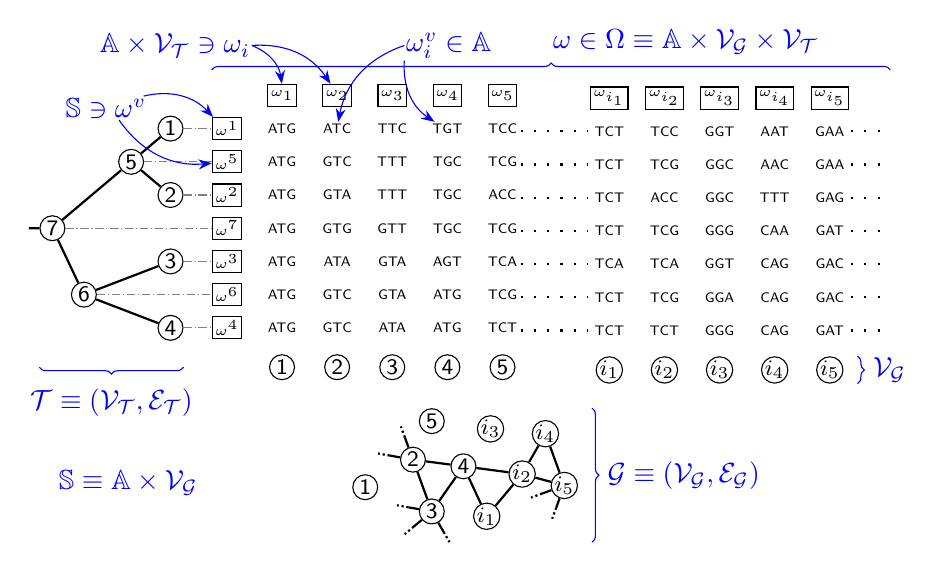
\begin{tikzpicture} 
[font=\tiny, label distance=0 cm, inner sep=0.5 pt,
every node/.style={anchor=center},
%every label/.style={blue},
itc/.style={blue!40!white, font={\rmfamily\tiny}},
otc/.style={black, font={\rmfamily\tiny}},
ita/.style={blue!40!white, font={\bfseries\tiny}},
ota/.style={black, font={\bfseries\tiny}},
]

% first block of alignment
\matrix[column sep={0.7 cm,between origins}, row sep={12 pt,between origins}] (codon-aln) at (0,0) {
\node (v0) {}; & \node[draw, minimum size=8 pt, inner sep=1 pt] (v0s1) {\(\omega_1\)}; & \node[draw, minimum size=8 pt, inner sep=1 pt] (v0s2) {\(\omega_2\)}; & \node[draw, minimum size=8 pt, inner sep=1 pt] (v0s3) {\(\omega_3\)}; & \node[draw, minimum size=8 pt, inner sep=1 pt] (v0s4) {\(\omega_4\)}; & \node[draw, minimum size=8 pt, inner sep=1 pt] (v0s5) {\(\omega_5\)}; \\
\node[draw, minimum size=8 pt, inner sep=1 pt] (v1) {\(\omega^1\)}; & \node (v1s1) {ATG}; & \node (v1s2) {ATC}; & \node (v1s3) {TTC}; & \node (v1s4) {TGT}; & \node (v1s5) {TCC}; \\
\node[draw, minimum size=8 pt, inner sep=1 pt] (v5) {\(\omega^5\)}; & \node {ATG}; & \node {GTC}; & \node {TTT}; & \node {TGC}; & \node {TCG}; \\
\node[draw, minimum size=8 pt, inner sep=1 pt] (v2) {\(\omega^2\)}; & \node {ATG}; & \node {GTA}; & \node {TTT}; & \node {TGC}; & \node {ACC}; \\
\node[draw, minimum size=8 pt, inner sep=1 pt] (v7) {\(\omega^7\)}; & \node {ATG}; & \node {GTG}; & \node {GTT}; & \node {TGC}; & \node {TCG}; \\
\node[draw, minimum size=8 pt, inner sep=1 pt] (v3) {\(\omega^3\)}; & \node {ATG}; & \node {ATA}; & \node {GTA}; & \node {AGT}; & \node {TCA}; \\
\node[draw, minimum size=8 pt, inner sep=1 pt] (v6) {\(\omega^6\)}; & \node {ATG}; & \node {GTC}; & \node {GTA}; & \node {ATG}; & \node {TCG}; \\
\node[draw, minimum size=8 pt, inner sep=1 pt] (v4) {\(\omega^4\)}; & \node (s1) {ATG}; & \node (s2) {GTC}; & \node (s3) {ATA}; & \node (s4) {ATG}; & \node (s5) {TCT}; \\ };

% second block of alignment
\matrix[column sep={0.7 cm,between origins}, row sep={12 pt,between origins}] (codon-aln-2) at (4.5 cm,0) {
\node[draw, minimum size=8 pt, inner sep=1 pt] {\(\omega_{i_1}\)}; & \node[draw, minimum size=8 pt, inner sep=1 pt] {\(\omega_{i_2}\)}; & \node[draw, minimum size=8 pt, inner sep=1 pt] {\(\omega_{i_3}\)}; & \node[draw, minimum size=8 pt, inner sep=1 pt] {\(\omega_{i_4}\)}; & \node[draw, minimum size=8 pt, inner sep=1 pt] {\(\omega_{i_5}\)}; \\
\node (w1) {TCT}; & \node {TCC}; & \node {GGT}; & \node {AAT}; & \node {GAA}; \\
\node (w5) {TCT}; & \node {TCG}; & \node {GGC}; & \node {AAC}; & \node {GAA}; \\
\node (w2) {TCT}; & \node {ACC}; & \node {GGC}; & \node {TTT}; & \node {GAG}; \\
\node (w7) {TCT}; & \node {TCG}; & \node {GGG}; & \node {CAA}; & \node {GAT}; \\
\node (w3) {TCA}; & \node {TCA}; & \node {GGT}; & \node {CAG}; & \node {GAC}; \\
\node (w6) {TCT}; & \node {TCG}; & \node {GGA}; & \node {CAG}; & \node {GAC}; \\
\node (w4) {TCT}; & \node (s7) {TCT}; & \node (s8) {GGG}; & \node (s9) {CAG}; & \node (s10) {GAT}; \\ };

% dotted lines after first block
\draw[thick, loosely dotted]
foreach \x in {1,...,4}
{
(codon-aln.east|-w\x) -- (codon-aln-2.west|-w\x)
(codon-aln-2.east|-w\x) -- +(0.5,0)
}
;

% dotted lines after second block
\draw[thick, loosely dotted]
foreach \x in {5,...,7}
{
(codon-aln.east|-w\x) -- (codon-aln-2.west|-w\x)
(codon-aln-2.east|-w\x) -- +(0.5,0) coordinate (s11)
}
;

\begin{scope}[font={\footnotesize}, every node/.style={draw, inner sep=0 pt, minimum size=9 pt,
circle, fill=white}]

% nodes of phylogeny
\path[draw]
foreach \x in {1,...,4}
{(v\x-|codon-aln.west) +(-0.5,0) node (V\x) {\x}}
(v5-|codon-aln.west) +(-1,0) node (V5) {5}
(v6-|codon-aln.west) +(-1.6,0) node (V6) {6}
(v7-|codon-aln.west) +(-2.0,0) node (V7) {7}
;

% draw phylogeny
\draw[thick]
(V7) -- (V5)
(V5) -- (V1)
(V5) -- (V2)
(V7) -- (V6)
(V6) -- (V3)
(V6) -- (V4)
(V7) -- +(-0.3,0)
;
\draw[thin, gray, densely dash dot]
foreach \x in {1,...,7}
{(V\x) -- (v\x)}
;

% site nodes to the bottom of columns
\path[]
%(v4) coordinate (s1)
(w4) coordinate (s6)
foreach \x in {1,...,5}
{(s\x) +(0,-0.5) node (S\x) {\x}}
foreach \x/\y in {6/1,7/2,8/3,9/4,10/5}
{(s\x) +(0,-0.5) node (S\x) {\(i_\y\)}}
(S10-|s11) coordinate (S11)
;

% SCHEMATI STRUCTURE
\begin{scope}[xshift=0.0 cm, yshift=-3.5 cm]

% position sites in schematic structure
\path
(0,0) coordinate (a1)
-- ++(30:0.7) coordinate (a2)
-- ++(-70:0.7) coordinate (a3)
-- ++(55:0.7) coordinate (a4)
-- ++(125:0.7) coordinate (a5)
(a3) ++(-5:0.7) coordinate (a6)
-- ++(50:0.7) coordinate (a7)
-- ++(125:0.7) coordinate (a8)
-- ++(-05:0.7) coordinate (a9)
-- ++(-70:0.7) coordinate (a10)
;

% site labels
\path[draw] foreach \x in {1,...,5}
{(a\x) node (A\x) {\x}}
;
\path[draw] foreach \x/\y in {6/1,7/2,8/3,9/4,10/5}
{(a\x) node (A\x) {\(i_\y\)}}
;

% site dependencies
\draw[thick]
(A2) -- coordinate (A2A3) (A3)
(A2) -- coordinate (A2A4) (A4)
(A3) -- (A4)
(A4) -- (A6)
(A4) -- (A7)
(A6) -- (A7)
(A7) -- (A9)
(A7) -- (A10)
(A9) -- (A10)
;

\path
(A2) ++(110:0.3 cm) coordinate (B2a) ++(110:0.15 cm) coordinate (C2a)
(A2) ++(170:0.3 cm) coordinate (B2b) ++(170:0.15 cm) coordinate (C2b)
(A3) ++(220:0.3 cm) coordinate (B3a) ++(220:0.15 cm) coordinate (C3a)
(A3) ++(170:0.3 cm) coordinate (B3b) ++(170:0.15 cm) coordinate (C3b)
(A3) ++(-60:0.3 cm) coordinate (B3c) ++(-60:0.15 cm) coordinate (C3c)
%(A9) ++(220:0.3 cm) coordinate (B9a) ++(220:0.15 cm) coordinate (C9a)
(A10) ++(250:0.3 cm) coordinate (B10a) ++(250:0.15 cm) coordinate (C10a)
(A10) ++(200:0.3 cm) coordinate (B10b) ++(200:0.15 cm) coordinate (C10b)
;

\draw[thick]
(A2) -- (B2a)
(A2) -- (B2b)
(A3) -- (B3a)
(A3) -- (B3b)
(A3) -- (B3c)
(A10) -- (B10a)
(A10) -- (B10b)
;

\draw[thick, densely dotted]
(B2a) -- (C2a)
(B2b) -- (C2b)
(B3a) -- (C3a)
(B3b) -- (C3b)
(B3c) -- (C3c)
(B10a) -- (C10a)
(B10b) -- (C10b)
;

\end{scope}
\end{scope}

\begin{scope}[blue, font=\normalsize]

% label for phylogeny
\draw[decorate, decoration={brace, mirror}]
(V7.west|-S1) --
node[below=7 pt, align=center] 
{\(\mathcal{T}\equiv(\mathcal{V}_\mathcal{T}, \mathcal{E}_\mathcal{T})\)}
(V1.east|-S1)
;

% label for site dependency graph
\draw[decorate, decoration={brace, raise=10 pt}]
(A10|-A5.north) --
node[right=15 pt, align=left]
{\(\mathcal{G}\equiv(\mathcal{V}_\mathcal{G}, \mathcal{E}_\mathcal{G})\)}
(A10|-C3c)
;

% label for sites
\draw[decorate, decoration={brace, raise=10 pt}]
(S10.north) --
node[right=15 pt, align=left] {\(\mathcal{V}_\mathcal{G}\)}
(S10.south)
;

% label for sequence family
\draw[decorate, decoration={brace, raise=5 pt}]
(v1.west|-v0s1.north) -- coordinate (m0) (s11|-v0s1.north)
(m0) +(0,10 pt) node[anchor=south west] {\(\omega \in \Omega\equiv
\mathbb{A} \times \mathcal{V}_\mathcal{G} \times \mathcal{V}_\mathcal{T} \)}
;

% labels for site patterns and sequences
\path
(v4) +(-100:2.0) node[anchor=east] (seq-space)
{\(\mathbb{S} \equiv \mathbb{A} \times \mathcal{V}_\mathcal{G}\)}
;

% labels for site patterns and sequences
\path
(v0s1) +(155:1.5 cm) node[align=right] (omega-i) {\( \mathbb{A} \times \mathcal{V}_\mathcal{T} \ni \omega_i \)}
(v1) +(170:1.5 cm) node[align=right] (omega-v) {\(\mathbb{S}\ni\omega^v\) }
(omega-i.east) +(2.5,0) node (omega-i-v) {\(\omega^v_i\in\mathbb{A}\)}
;

\draw[thin, -Stealth] (omega-i.east) to[bend left] (v0s1) ;
\draw[thin, -Stealth] (omega-i.east) to[bend left] (v0s2) ;

\draw[thin, -Stealth] (omega-v) to[bend left] (v1) ;
\draw[thin, -Stealth] (omega-v) to[bend right] (v5) ;

\draw[thin, -Stealth] (omega-i-v.west) to[bend right] (v1s2) ;
\draw[thin, -Stealth] (omega-i-v.south west) to[bend right] (v1s4) ;

\end{scope}

\end{tikzpicture}
\end{document}








